\chapter{Projektplan}
\section{Änderungsgeschichte}
\begin{tabularx}{\textwidth}{|c|c|X|c|}
  \hline
  \textbf{Datum} & \textbf{Version} & \textbf{Änderung} & \textbf{Autor} \\
  \hline \hline
  26.02.2016 & 1.0 & Erstellen des Projektplans & Martin Stypinski \\
  \hline
\end{tabularx}

\section{Einleitung}
\subsection{Ziel und Zweck}
Ziel dieser Arbeit ist \textit{Project-Helin} umzusetzten. 

\subsection{Lieferumfang}
Der Lieferumfang dieser Arbeit entspricht den Vorgaben der HSR:
\begin{itemize}
	\item{Zu Handen des Betreuers:
	\begin{itemize}
		\item{Ein gedrucktes Exemplar der Dokumentation}
		\item{Dokumentation, sämtliche Dokumente und Sourcen auf CD}
	\end{itemize}}
	\item{Poster - Enthält Zusammenfassung der Arbeit}
	\item{Abstract für die Bachelorarbeitsbrochure}
\end{itemize}
Zusätzlich ist es uns ein Anliegen, dass der Sourcecode und die Erfahrungen über den Zeitraum der Bachelorarbeit hinaus bestehen bleiben. Daher wurde ein github-repository eingerichtet, dass nach beendigung der Arbeit sämtliche Teile enthält: \textbf{\url{https://github.com/Project-Helin}}

\subsection{Annahmen und Einschränkungen}
Es kann angenommen werden, dass der Zeitplan im Rahmen der regulären Bachelorarbeit Zeit gültig ist. Es wird dabei berücksichtigt das ein Zeithorizont von 17 Wochen zuverfügung steht und die maximale Arbeitszeit von 360 Stunden pro Person nicht überschritten werden soll.

\section{Projektorganisation}
\subsection{Organisationsstruktur}
\begin{tabularx}{\textwidth}{|c|c|X|}
  \hline
  \textbf{Name} & \textbf{E-Mail} & \textbf{Verantwortung} \\
  \hline \hline
  Prof. Dr. Markus Stolz & \url{markus.stolze@hsr.ch} & Betreuer der Arbeit\\
  \hline \hline
  Marcel Amsler & \url{marcel.amsler@hsr.ch} & \\
  \hline
  Kirusanth Poopolasingam & \url{kirusanth.poopalasingam@hsr.ch} & \\
  \hline
  Martin Stypinski & \url{martin.stypinski@hsr.ch} & \\
    \hline
\end{tabularx}

\section{Risikomanagement}
\subsection{Risiken}
\LTXtable{\textwidth}{risk.tex}

\subsection{Umgang mit Risiken}
\begin{figure}[htbp]
\centering
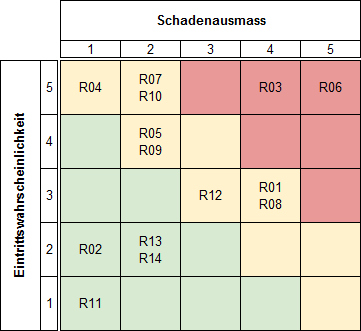
\includegraphics{images/risk_result.png}
\caption{Risiko Matrix}
\label{Risk result}
\end{figure}


\subsection{Massnahmen}

\section{Meilensteinplanung}